\documentclass[letterpaper,10pt,titlepage]{article}

\usepackage{amsmath}                                         
\usepackage{amsthm}

\usepackage{alltt}                                           
\usepackage{float}
\usepackage{color}

\usepackage{balance}
\usepackage[TABBOTCAP, tight]{subfigure}
\usepackage{enumitem}

\usepackage{pstricks, pst-node}
\usepackage{geometry}
\geometry{textheight=10in, textwidth=7.5in}
\usepackage{graphicx}
%random comment

\newcommand{\cred}[1]{{\color{red}#1}}
\newcommand{\cblue}[1]{{\color{blue}#1}}

\usepackage{hyperref}

\def\name{David Merrick}


%% The following metadata will show up in the PDF properties
\hypersetup{
  colorlinks = true,
  urlcolor = black,
  pdfauthor = {\name},
  pdfkeywords = {cs311 ``operating systems'' pipes signals},
  pdftitle = {CS 311 Project 3: Uniqify},
  pdfsubject = {CS 311 Project 3},
  pdfpagemode = UseNone
}

\parindent = 0.0 in
\parskip = 0.2 in

\begin{document}
David Merrick

CS 311

15 February, 2013

\begin{center}
{\LARGE Timing Plots for Assignment 3}
\end{center}

\begin{figure}[H]
	\begin{center}
	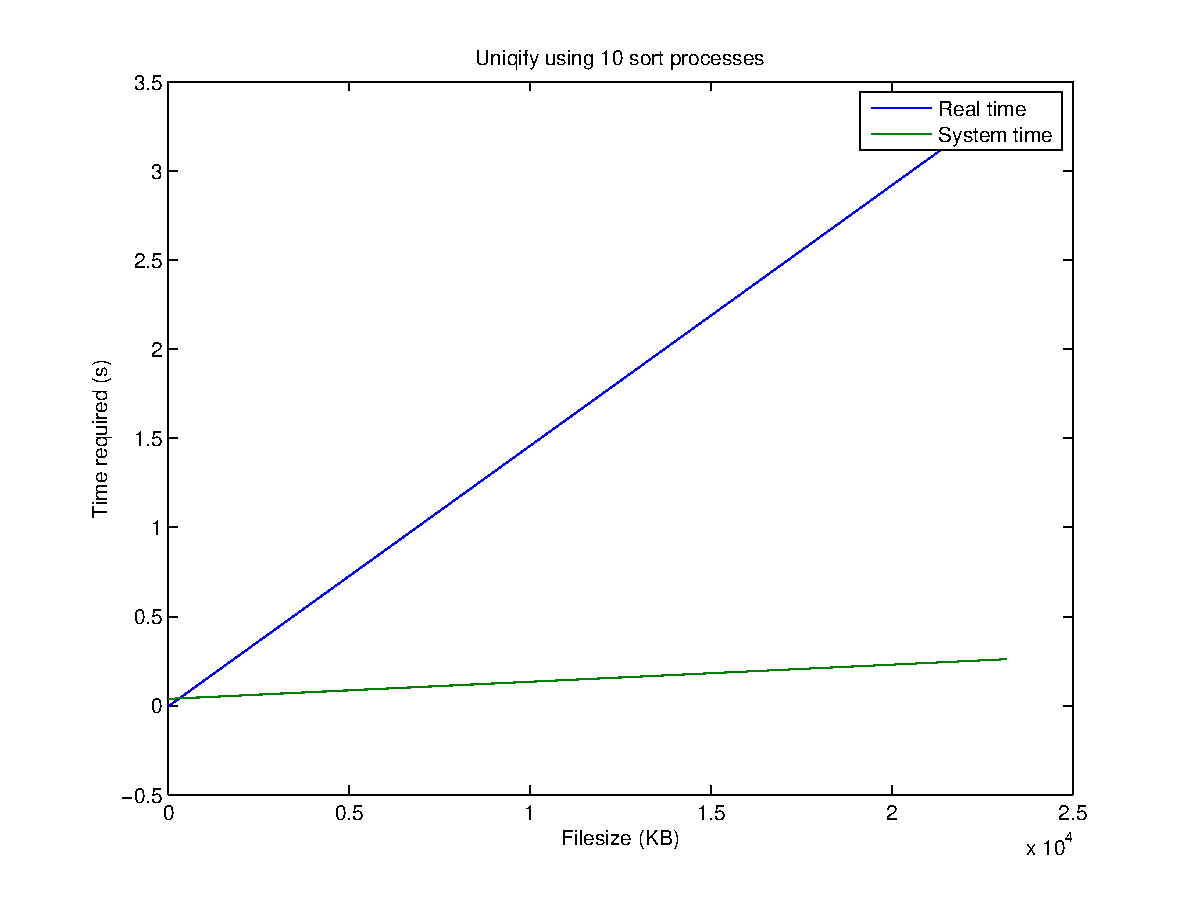
\includegraphics[width=8in]{figure1}
	\end{center}
	\caption{Uniqify using 10 sort processes.}
\end{figure}
\begin{figure}[H]
	\begin{center}
	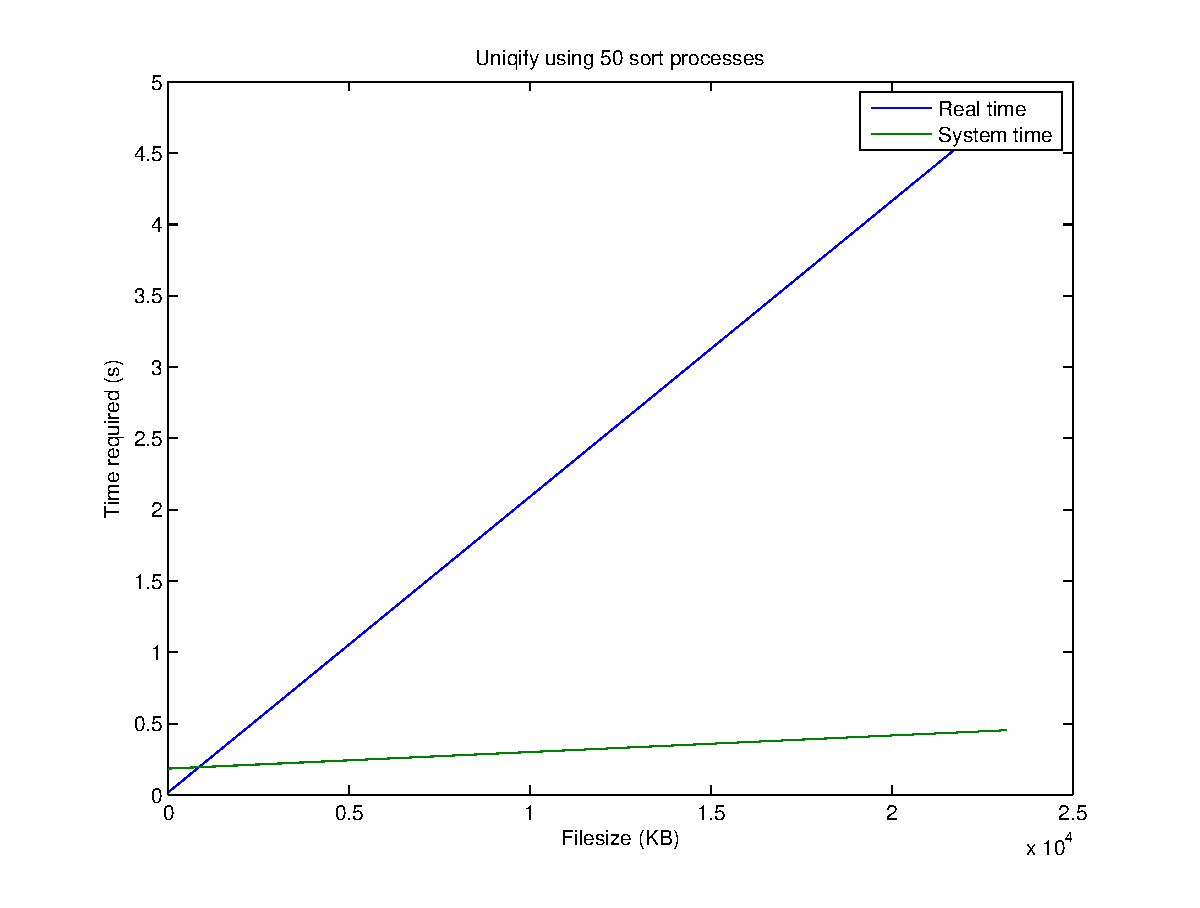
\includegraphics[width=8in]{figure2}
	\end{center}
	\caption{Uniqify using 50 sort processes.}
\end{figure}
\begin{figure}[H]
	\begin{center}
	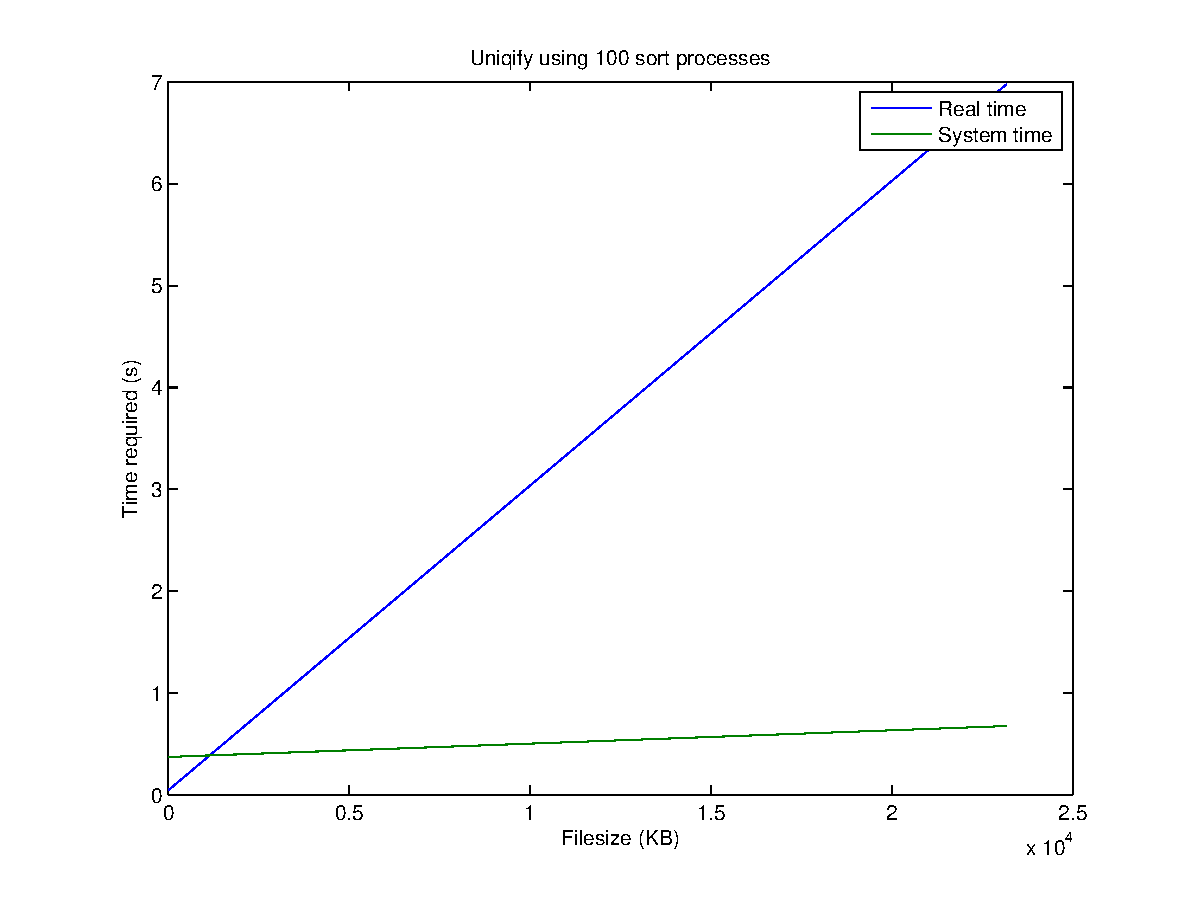
\includegraphics[width=8in]{figure3}
	\end{center}
	\caption{Uniqify using 100 sort processes.}
\end{figure}
%input the pygmentized output of mt19937ar.c, using a (hopefully) unique name
%this file only exists at compile time. Feel free to change that.
%\input{__mt.h.tex}
\end{document}
